% =============================================================================
%  Sparse Grassmann LLM — Edge-Device Efficiency Study
%  Full Technical Report (IEEE Conference Format)
% =============================================================================
\documentclass[conference]{IEEEtran}
\IEEEoverridecommandlockouts

% ── Packages ─────────────────────────────────────────────────────────────────
\usepackage[utf8]{inputenc}
\usepackage[T1]{fontenc}
\usepackage{lmodern}
\usepackage{amsmath,amssymb,amsfonts}
\usepackage{graphicx}
\usepackage{booktabs}
\usepackage{multirow}
\usepackage{caption}
\usepackage{subcaption}
\usepackage{hyperref}
\usepackage{xcolor}
\usepackage{enumitem}
\usepackage{algorithm}
\usepackage{algorithmic}
\usepackage{tabularx}
\usepackage{siunitx}
\usepackage{cite} % Replaced natbib with cite for IEEE format

% ── TikZ (required for architecture diagrams) ────────────────────────────────
\usepackage{tikz}
\usetikzlibrary{
  shapes.geometric,
  arrows.meta,
  positioning,
  fit,
  calc,
  decorations.pathreplacing,
  decorations.markings
}
\usepackage{pifont}   % for \ding numerals used in figure captions

% ── TikZ node styles ─────────────────────────────────────────────────────────
\tikzset{
  arrow/.style    = {-{Stealth[length=6pt]}, thick},
  residual/.style = {-{Stealth[length=5pt]}, thick, dashed, gray!60},
  brace/.style    = {decorate,
                     decoration={brace, amplitude=5pt, mirror},
                     thick, gray!70},
  ioblock/.style  = {draw, rounded corners=4pt, fill=gray!12,
                     minimum height=0.75cm, align=center,
                     font=\small\sffamily, thick},
  gblock/.style   = {draw, rounded corners=4pt, fill=teal!18,
                     minimum height=0.75cm, align=center,
                     font=\small\sffamily, thick},
  tblock/.style   = {draw, rounded corners=4pt, fill=orange!18,
                     minimum height=0.75cm, align=center,
                     font=\small\sffamily, thick},
  sblock/.style   = {draw, rounded corners=4pt, fill=violet!18,
                     minimum height=0.75cm, align=center,
                     font=\small\sffamily, thick},
  sparsenode/.style = {draw, minimum size=0.4cm, inner sep=1pt,
                       font=\tiny\sffamily},
}

% ── Formatting ───────────────────────────────────────────────────────────────
\hypersetup{
  colorlinks=true,
  linkcolor=blue!70!black,
  citecolor=green!50!black,
  urlcolor=blue!60!black,
}
\sisetup{group-separator={,}, group-minimum-digits=4}
\captionsetup{font=small, labelfont=bf}

% ── Macros ───────────────────────────────────────────────────────────────────
\newcommand{\grassmann}{\textsc{Grassmann}}
\newcommand{\pat}{\textsc{PAT}}
\newcommand{\ppl}{\mathrm{PPL}}
\newcommand{\seqlen}{\ensuremath{n}}
\newcommand{\bigO}[1]{\ensuremath{\mathcal{O}(#1)}}

% ═════════════════════════════════════════════════════════════════════════════
\begin{document}

\title{%
  Sparse Grassmann LLM: Grassmann-Flow Mixing with 2:4 Structured Sparsity for Edge-Device Language Modelling
}

\author{
\IEEEauthorblockN{Adithya MS}
\IEEEauthorblockA{\textit{Department of Computer Science} \\
\textit{IIITDM Kancheepuram}\\
Chennai, India}
\and
\IEEEauthorblockN{Dr. Nachiketa Mishra}
\IEEEauthorblockA{\textit{Department of Mathematics} \\
\textit{IIITDM Kancheepuram}\\
Chennai, India}
}

\maketitle

% ═════════════════════════════════════════════════════════════════════════════
\begin{abstract}
We present a comparative study of a \grassmann{}-flow language model with
2:4 structured sparsity and Pruning-Aware Training (\pat{}) against a dense
GPT-2-style Transformer baseline at matched parameter count
($\sim$22.5\,M). All models are trained on Wikitext-2 at a sequence length
of 2048 tokens.

Our experiments show that \grassmann{} mixing—which replaces quadratic
self-attention with \bigO{n} causal linear mixing derived from Pl\"ucker
coordinates on the Grassmann manifold—achieves \textbf{3.7$\times$ lower
perplexity} (139 vs.\ 517), \textbf{2$\times$ higher throughput} at
\seqlen{}=2048, and \textbf{2$\times$ less VRAM} than the Transformer,
with no key-value cache required. Under INT8 dynamic quantisation on CPU
(the edge-device regime), \grassmann{}+\pat{} delivers 2.4$\times$ more
tokens per second than the Transformer at dramatically better quality.
These results position \grassmann{}-flow mixing as a compelling
alternative for memory- and compute-constrained deployment.
\end{abstract}

\begin{IEEEkeywords}
Grassmann manifold, language modelling, structured sparsity, edge computing, efficient inference.
\end{IEEEkeywords}

% ═════════════════════════════════════════════════════════════════════════════
\section{Introduction}
\label{sec:intro}

Standard Transformer language models carry two inference costs that are
problematic on edge devices:

\begin{enumerate}[leftmargin=*,topsep=3pt,itemsep=2pt]
  \item \textbf{Quadratic attention.} Self-attention computes
        $\bigO{n^{2}}$ dot products per layer, where $n$ is the
        sequence length. At long contexts this dominates both latency
        and memory.
  \item \textbf{KV-cache memory.} Autoregressive generation caches the
        key and value projections for every past token. For a model
        with $L$ layers, $H$ heads, and head dimension $d_h$, the
        KV-cache grows as $2 L H n d_h$ floats—tens or hundreds of MB
        at long contexts.
\end{enumerate}

\grassmann{}-flow mixing~\cite{grassmann2024} replaces self-attention
with a \textbf{causal linear mixing} operation derived from Pl\"ucker
coordinates on the Grassmannian. While standard attention scales quadratically
with the sequence length $n$, each \grassmann{} layer scales linearly as
\bigO{n \cdot d}. The hidden dimension $d$ (specifically $d_{\text{model}} = 512$ in our study)
represents the width of the feature vector for each token; it acts as the
latent space where semantic and syntactic information is encoded before
being mixed by the \grassmann{} flow.
Furthermore, this architecture requires \emph{no KV-cache}, making the
inference memory footprint effectively independent of sequence length
during autoregressive generation.

On top of the architectural change, we apply \textbf{2:4 structured
(semi-structured) sparsity}~\cite{nvidia2to4} to all feed-forward weight
matrices. Exactly 2 out of every 4 weights per row are zeroed, reducing
effective weight storage by 50\%. On Ampere+ GPUs this maps to the
Sparse Tensor Core path for up to 2$\times$ throughput; even without
that hardware path, 50\% fewer non-zero weights reduce memory bandwidth
pressure.

\paragraph{Contributions.}
\begin{enumerate}[leftmargin=*,topsep=3pt,itemsep=2pt]
  \item A matched-parameter ($\sim$22.5\,M) comparison of \grassmann{}
        mixing vs.\ a GPT-2-style Transformer on Wikitext-2 at
        $n = 2048$.
  \item A dense ablation isolating the architectural benefit of
        \grassmann{} mixing from the sparsity benefit of \pat{}.
  \item Comprehensive inference benchmarks: FP32 GPU throughput, peak
        VRAM scaling, latency, and INT8 dynamic quantisation on CPU
        across sequence lengths 64--2048.
\end{enumerate}


% ═════════════════════════════════════════════════════════════════════════════
\section{Architecture Diagrams}
\label{sec:diagrams}

This section provides a detailed walkthrough of both architectures
compared in this study. Figure~\ref{fig:arch-compare} shows the
high-level block diagrams side by side.

% ─────────────────────────────────────────────────────────────────────────────
%  FIGURE: Side-by-side architecture diagrams (Spans Two Columns)
% ─────────────────────────────────────────────────────────────────────────────
\begin{figure*}[t]
\centering
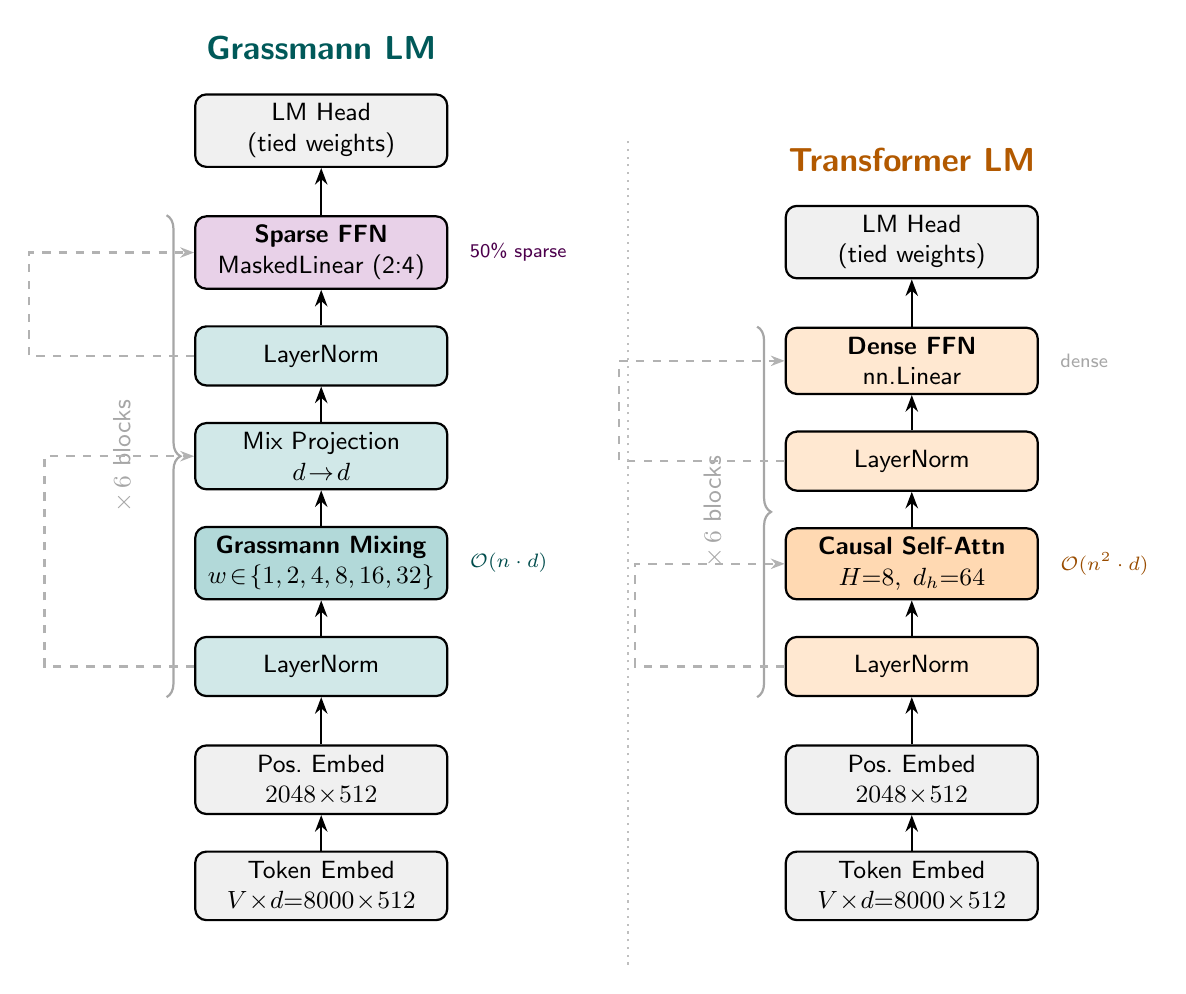
\begin{tikzpicture}[node distance=0.45cm]

% ========== LEFT: Grassmann LM ==========
\begin{scope}[local bounding box=grassmann]
  \node[ioblock, minimum width=3.2cm] (gemb) {Token Embed\\$V \!\times\! d{=}8000 \!\times\! 512$};
  \node[ioblock, minimum width=3.2cm, above=of gemb] (gpos) {Pos.\ Embed\\$2048 \!\times\! 512$};

  \node[gblock, above=0.6cm of gpos, minimum width=3.2cm] (gln1) {LayerNorm};
  \node[gblock, above=of gln1, minimum width=3.2cm, fill=teal!30] (gmix)
    {\textbf{Grassmann Mixing}\\$w\!\in\!\{1,2,4,8,16,32\}$};
  \node[gblock, above=of gmix, minimum width=3.2cm] (gmixproj) {Mix Projection\\$d \!\to\! d$};
  \node[gblock, above=of gmixproj, minimum width=3.2cm] (gln2) {LayerNorm};
  \node[sblock, above=of gln2, minimum width=3.2cm] (gffn)
    {\textbf{Sparse FFN}\\MaskedLinear (2:4)};

  \draw[brace] ([xshift=-0.35cm]gln1.south west) -- ([xshift=-0.35cm]gffn.north west)
    node[midway, left=0.3cm, font=\small\sffamily, rotate=90, anchor=south] {$\times\,6$ blocks};

  \coordinate (gres1) at ([xshift=-1.9cm]gmix.west);
  \draw[residual] (gln1.west) -| (gres1) |- (gmixproj.west);
  \coordinate (gres2) at ([xshift=-2.1cm]gffn.west);
  \draw[residual] (gln2.west) -| (gres2) |- (gffn.west);

  \node[ioblock, above=0.6cm of gffn, minimum width=3.2cm] (ghead) {LM Head\\(tied weights)};

  \draw[arrow] (gemb) -- (gpos);
  \draw[arrow] (gpos) -- (gln1);
  \draw[arrow] (gln1) -- (gmix);
  \draw[arrow] (gmix) -- (gmixproj);
  \draw[arrow] (gmixproj) -- (gln2);
  \draw[arrow] (gln2) -- (gffn);
  \draw[arrow] (gffn) -- (ghead);

  \node[above=0.3cm of ghead, font=\large\bfseries\sffamily, teal!70!black]
    (gtitle) {\grassmann{} LM};

  \node[right=0.15cm of gmix, font=\scriptsize\sffamily, teal!60!black]
    {$\bigO{n \cdot d}$};
  \node[right=0.15cm of gffn, font=\scriptsize\sffamily, violet!60!black]
    {50\% sparse};
\end{scope}

% ========== RIGHT: Transformer LM ==========
\begin{scope}[xshift=7.5cm, local bounding box=transformer]
  \node[ioblock, minimum width=3.2cm] (temb) {Token Embed\\$V \!\times\! d{=}8000 \!\times\! 512$};
  \node[ioblock, minimum width=3.2cm, above=of temb] (tpos) {Pos.\ Embed\\$2048 \!\times\! 512$};

  \node[tblock, above=0.6cm of tpos, minimum width=3.2cm] (tln1) {LayerNorm};
  \node[tblock, above=of tln1, minimum width=3.2cm, fill=orange!30] (tattn)
    {\textbf{Causal Self-Attn}\\$H{=}8,\; d_h{=}64$};
  \node[tblock, above=of tattn, minimum width=3.2cm] (tln2) {LayerNorm};
  \node[tblock, above=of tln2, minimum width=3.2cm] (tffn)
    {\textbf{Dense FFN}\\nn.Linear};

  \draw[brace] ([xshift=-0.35cm]tln1.south west) -- ([xshift=-0.35cm]tffn.north west)
    node[midway, left=0.3cm, font=\small\sffamily, rotate=90, anchor=south] {$\times\,6$ blocks};

  \coordinate (tres1) at ([xshift=-1.9cm]tattn.west);
  \draw[residual] (tln1.west) -| (tres1) |- (tattn.west);
  \coordinate (tres2) at ([xshift=-2.1cm]tffn.west);
  \draw[residual] (tln2.west) -| (tres2) |- (tffn.west);

  \node[ioblock, above=0.6cm of tffn, minimum width=3.2cm] (thead) {LM Head\\(tied weights)};

  \draw[arrow] (temb) -- (tpos);
  \draw[arrow] (tpos) -- (tln1);
  \draw[arrow] (tln1) -- (tattn);
  \draw[arrow] (tattn) -- (tln2);
  \draw[arrow] (tln2) -- (tffn);
  \draw[arrow] (tffn) -- (thead);

  \node[above=0.3cm of thead, font=\large\bfseries\sffamily, orange!70!black]
    (ttitle) {Transformer LM};

  \node[right=0.15cm of tattn, font=\scriptsize\sffamily, orange!60!black]
    {$\bigO{n^2 \cdot d}$};
  \node[right=0.15cm of tffn, font=\scriptsize\sffamily, gray!70]
    {dense};
\end{scope}

% Dividing line
\draw[thick, dotted, gray!50] (3.9, -1) -- (3.9, 9.5);

\end{tikzpicture}
\caption{%
  \textbf{Side-by-side architecture comparison.}
  \emph{Left:}~\grassmann{} LM replaces self-attention with
  $\bigO{n \cdot d}$ Grassmann mixing and uses 2:4 sparse FFN layers.
  \emph{Right:}~Transformer LM uses standard $\bigO{n^2 \cdot d}$
  causal self-attention with dense FFN layers.
  Both share 6 blocks, $d{=}512$, tied token embeddings,
  and pre-LayerNorm residual connections.
  Dashed arrows denote residual skip connections.%
}
\label{fig:arch-compare}
\end{figure*}


% ─────────────────────────────────────────────────────────────────────────────
%  FIGURE: Grassmann Mixing Layer detail
% ─────────────────────────────────────────────────────────────────────────────
\begin{figure}[htbp]
\centering
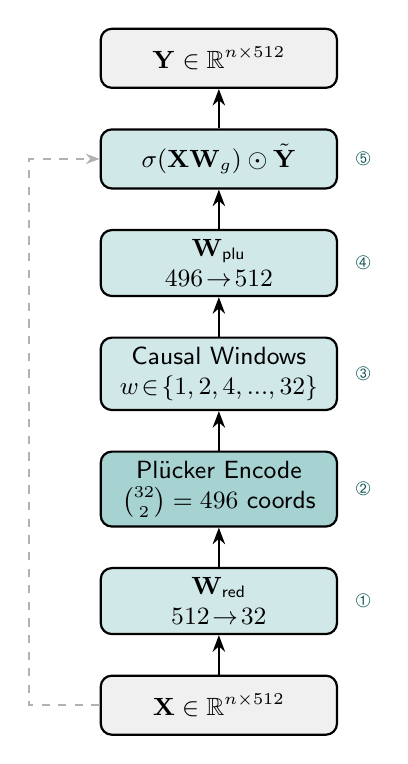
\begin{tikzpicture}[node distance=0.5cm, every node/.style={font=\small\sffamily}]

  \node[ioblock, minimum width=3.0cm] (inp)
    {$\mathbf{X} \in \mathbb{R}^{n \times 512}$};

  \node[gblock, above=0.5cm of inp, minimum width=3.0cm] (wred)
    {$\mathbf{W}_{\text{red}}$\\$512 \!\to\! 32$};
  \node[right=0.1cm of wred, font=\scriptsize, teal!60!black] {\ding{192}};

  \node[gblock, above=of wred, minimum width=3.0cm, fill=teal!35] (plu)
    {Pl\"ucker Encode\\$\binom{32}{2} = 496$ coords};
  \node[right=0.1cm of plu, font=\scriptsize, teal!60!black] {\ding{193}};

  \node[gblock, above=of plu, minimum width=3.0cm] (win)
    {Causal Windows\\$w\!\in\!\{1,2,4,...,32\}$};
  \node[right=0.1cm of win, font=\scriptsize, teal!60!black] {\ding{194}};

  \node[gblock, above=of win, minimum width=3.0cm] (wplu)
    {$\mathbf{W}_{\text{plu}}$\\$496 \!\to\! 512$};
  \node[right=0.1cm of wplu, font=\scriptsize, teal!60!black] {\ding{195}};

  \node[gblock, above=of wplu, minimum width=3.0cm] (gate)
    {$\sigma(\mathbf{X}\mathbf{W}_g) \odot \tilde{\mathbf{Y}}$};
  \node[right=0.1cm of gate, font=\scriptsize, teal!60!black] {\ding{196}};

  \node[ioblock, above=0.5cm of gate, minimum width=3.0cm] (out)
    {$\mathbf{Y} \in \mathbb{R}^{n \times 512}$};

  \draw[arrow] (inp) -- (wred);
  \draw[arrow] (wred) -- (plu);
  \draw[arrow] (plu) -- (win);
  \draw[arrow] (win) -- (wplu);
  \draw[arrow] (wplu) -- (gate);
  \draw[arrow] (gate) -- (out);

  \draw[residual] (inp.west) -- +(-0.9,0) |- (gate.west);

\end{tikzpicture}
\caption{%
  \textbf{Grassmann Mixing Layer} (one sublayer within a block).
  \ding{192}~Dimensionality reduction to $r{=}32$.
  \ding{193}~Pl\"ucker coordinate encoding on $\mathrm{Gr}(2,r)$.
  \ding{194}~Multi-scale causal windowing.
  \ding{195}~Back-projection to $d{=}512$.
  \ding{196}~Sigmoid gating.
  The dashed arrow carries the original input to the gate.
  Total cost: $\bigO{n \cdot d}$, \textbf{no KV-cache}.%
}
\label{fig:mixing-detail}
\end{figure}


% ─────────────────────────────────────────────────────────────────────────────
%  FIGURE: 2:4 Sparsity Pattern
% ─────────────────────────────────────────────────────────────────────────────
\begin{figure}[htbp]
\centering
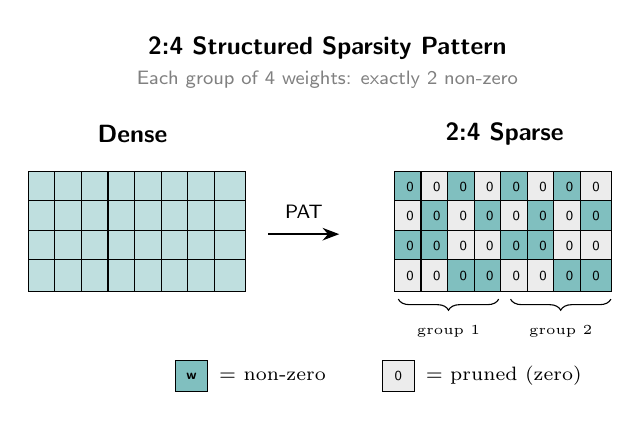
\begin{tikzpicture}[scale=0.75, every node/.style={font=\tiny\sffamily}] % Scaled down slightly for column fit

    % Header text
    \node[anchor=south, font=\small\sffamily\bfseries] at (4.8, 6.2) {2:4 Structured Sparsity Pattern};
    \node[anchor=south, font=\scriptsize\sffamily, gray] at (4.8, 5.7) {Each group of 4 weights: exactly 2 non-zero};

    % --- LEFT: DENSE MATRIX ---
    \node[font=\small\sffamily\bfseries] at (1.5, 5.1) {Dense};
    \foreach \r in {0,...,3} {
        \foreach \c in {0,...,7} {
            \node[sparsenode, fill=teal!25] at (\c*0.45, 4.2-\r*0.5) {};
        }
    }

    % --- CENTER: TRANSITION ARROW ---
    \draw[-{Stealth[length=6pt]}, thick] (3.8, 3.4) -- (5.0, 3.4)
        node[midway, above=2pt, font=\scriptsize\sffamily] {PAT};

    % --- RIGHT: SPARSE MATRIX ---
    \node[font=\small\sffamily\bfseries] at (7.8, 5.1) {2:4 Sparse};

    % Sparse Row 0
    \foreach \c/\txt/\clr in {0/w/teal!50, 1/0/gray!15, 2/w/teal!50, 3/0/gray!15, 4/w/teal!50, 5/0/gray!15, 6/w/teal!50, 7/0/gray!15}
        \node[sparsenode, fill=\clr] at (6.2+\c*0.45, 4.2) {\ifx\txt\w\textbf{w}\else 0\fi};

    % Sparse Row 1
    \foreach \c/\txt/\clr in {0/0/gray!15, 1/w/teal!50, 2/0/gray!15, 3/w/teal!50, 4/0/gray!15, 5/w/teal!50, 6/0/gray!15, 7/w/teal!50}
        \node[sparsenode, fill=\clr] at (6.2+\c*0.45, 3.7) {\ifx\txt\w\textbf{w}\else 0\fi};

    % Sparse Row 2
    \foreach \c/\txt/\clr in {0/w/teal!50, 1/w/teal!50, 2/0/gray!15, 3/0/gray!15, 4/w/teal!50, 5/w/teal!50, 6/0/gray!15, 7/0/gray!15}
        \node[sparsenode, fill=\clr] at (6.2+\c*0.45, 3.2) {\ifx\txt\w\textbf{w}\else 0\fi};

    % Sparse Row 3
    \foreach \c/\txt/\clr in {0/0/gray!15, 1/0/gray!15, 2/w/teal!50, 3/w/teal!50, 4/0/gray!15, 5/0/gray!15, 6/w/teal!50, 7/w/teal!50}
        \node[sparsenode, fill=\clr] at (6.2+\c*0.45, 2.7) {\ifx\txt\w\textbf{w}\else 0\fi};

    % Group braces
    \draw[decorate, decoration={brace, amplitude=4pt, mirror}]
        (6.0, 2.3) -- (7.7, 2.3) node[midway, below=6pt, font=\tiny] {group 1};
    \draw[decorate, decoration={brace, amplitude=4pt, mirror}]
        (7.9, 2.3) -- (9.6, 2.3) node[midway, below=6pt, font=\tiny] {group 2};

    % --- LEGEND: Fixed coordinate syntax ---
    \begin{scope}[yshift=0.5cm]
        \node[sparsenode, fill=teal!50] (leg1) at (2.5, 0.5) {\textbf{w}};
        \node[anchor=west, font=\scriptsize] at (2.8, 0.5) {= non-zero};
        
        \node[sparsenode, fill=gray!15] (leg2) at (6.0, 0.5) {0};
        \node[anchor=west, font=\scriptsize] at (6.3, 0.5) {= pruned (zero)};
    \end{scope}

\end{tikzpicture}
\caption{\textbf{2:4 Structured Sparsity Pattern.} During Pruning-Aware Training (PAT), the model learns to maintain exactly 50\% sparsity in a block-structured format.}
\label{fig:sparsity}
\end{figure}


% ─────────────────────────────────────────────────────────────────────────────
%  FIGURE: Multi-Scale Causal Windows
% ─────────────────────────────────────────────────────────────────────────────
\begin{figure}[htbp]
\centering
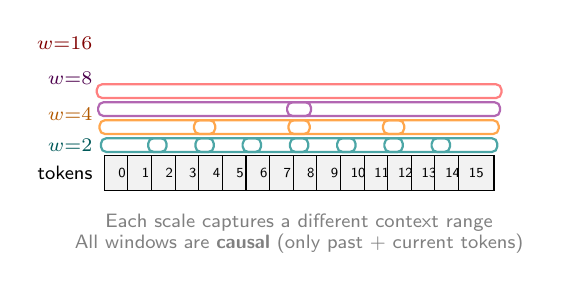
\begin{tikzpicture}[scale=0.5, every node/.style={font=\tiny\sffamily}]

    % Tokens Base Row
    \foreach \t in {0,...,15} {
        \node[draw, minimum size=0.45cm, fill=gray!10, inner sep=0pt]
            (t\t) at (\t*0.6, 0) {\t};
    }
    \node[font=\scriptsize\sffamily, anchor=east] at (-0.5, 0) {tokens};

    % Window Scale w=2 (Bottom Scale)
    \foreach \s in {0,2,...,14} {
        \pgfmathtruncatemacro{\e}{\s+1}
        \draw[thick, teal!70, rounded corners=2pt]
            ([xshift=-2pt, yshift=2pt]t\s.north west)
            rectangle
            ([xshift=2pt, yshift=12pt]t\e.north east);
    }
    \node[font=\scriptsize\sffamily, teal!70!black, anchor=east] at (-0.5, 0.7) {$w{=}2$};

    % Window Scale w=4 (Middle-Bottom)
    \foreach \s in {0,4,...,12} {
        \pgfmathtruncatemacro{\e}{\s+3}
        \draw[thick, orange!70, rounded corners=2pt]
            ([xshift=-3pt, yshift=15pt]t\s.north west)
            rectangle
            ([xshift=3pt, yshift=25pt]t\e.north east);
    }
    \node[font=\scriptsize\sffamily, orange!70!black, anchor=east] at (-0.5, 1.5) {$w{=}4$};

    % Window Scale w=8 (Middle-Top)
    \foreach \s in {0,8} {
        \pgfmathtruncatemacro{\e}{\s+7}
        \draw[thick, violet!60, rounded corners=2pt]
            ([xshift=-4pt, yshift=28pt]t\s.north west)
            rectangle
            ([xshift=4pt, yshift=38pt]t\e.north east);
    }
    \node[font=\scriptsize\sffamily, violet!60!black, anchor=east] at (-0.5, 2.4) {$w{=}8$};

    % Window Scale w=16 (Top Scale)
    \draw[thick, red!50, rounded corners=2pt]
        ([xshift=-5pt, yshift=41pt]t0.north west)
        rectangle
        ([xshift=5pt, yshift=51pt]t15.north east);
    \node[font=\scriptsize\sffamily, red!50!black, anchor=east] at (-0.5, 3.3) {$w{=}16$};

    % Bottom Annotations
    \node[font=\scriptsize\sffamily, gray, anchor=north] at (4.5, -0.8)
        {Each scale captures a different context range};
    \node[font=\scriptsize\sffamily, gray, anchor=north] at (4.5, -1.3)
        {All windows are \textbf{causal} (only past + current tokens)};

\end{tikzpicture}
\caption{\textbf{Multi-scale causal windows} in Grassmann mixing.}
\label{fig:windows}
\end{figure}


% ═════════════════════════════════════════════════════════════════════════════
\section{Architecture}
\label{sec:arch}

\subsection{Grassmann LM}

The \grassmann{} language model stacks 6 identical blocks, each
containing a \grassmann{} mixing sublayer followed by a sparse
feed-forward sublayer, with pre-LayerNorm residual connections.

\paragraph{Token representation.}
Tokens from a BPE vocabulary of 8\,000 are embedded into
$d_{\text{model}} = 512$ dimensions with a learned positional embedding
of length 2048. The output LM head is weight-tied to the token
embedding.

\paragraph{Grassmann Mixing.}
Given an input sequence $\mathbf{X} \in \mathbb{R}^{n \times d}$, each \grassmann{} mixing sublayer performs a series of transformations to integrate context without the need for quadratic attention:

\begin{enumerate}[leftmargin=*,topsep=4pt,itemsep=6pt]
    \item \textbf{Reduce}: The input is first projected into a lower-dimensional subspace $\mathbf{H} = \mathbf{X} \mathbf{W}_{\text{red}}$, where $\mathbf{W}_{\text{red}} \in \mathbb{R}^{d \times r}$ and the bottleneck rank $r = 32$.

    \item \textbf{Pl\"ucker Encode}: To map the reduced representation onto the Grassmannian manifold $\mathbf{Gr}(2, r)$, we compute the exterior product of the subspace coordinates. For each token, we extract all $\binom{r}{2} = 496$ unique pairs of indices $(i, j)$ from the vector $h \in \mathbb{R}^r$ to form the Pl\"ucker coordinates $p_{ij}$:
    \begin{equation}
        p_{ij} = \det \begin{pmatrix} h_i & h_j \\ \lambda_i & \lambda_j \end{pmatrix} = h_i \lambda_j - h_j \lambda_i
    \end{equation}
    where $\lambda$ represents a learned anchor parameter. The resulting vector $\mathbf{p} \in \mathbb{R}^{n \times 496}$ is $L_2$-normalised to ensure the representation resides on the unit hypersphere of the embedding space.

    \item \textbf{Project Back}: The geometric representation is projected back to the model's hidden dimension: $\tilde{\mathbf{Y}} = \mathbf{p}\mathbf{W}_{\text{plu}}$, where $\mathbf{W}_{\text{plu}} \in \mathbb{R}^{496 \times d}$.

    \item \textbf{Causal Multi-scale Blending}: To integrate temporal context, we apply six concurrent window sizes $w \in \{1, 2, 4, 8, 16, 32\}$. For each window, a causal cumulative sum computes a running average of the projected representations. The final output is a gated weighted sum of these windows, controlled by learned scalar coefficients.

    \item \textbf{Normalization}: A final \texttt{LayerNorm} is applied to the mixed output before the residual summation.
\end{enumerate}

This entire operation maintains a complexity of $\mathcal{O}(n \cdot d)$ per layer. Unlike standard Transformers, there are no $n \times n$ attention matrices, and the architecture requires no KV-cache during inference, ensuring memory consumption remains constant regardless of sequence length.

\paragraph{Sparse Feed-Forward (MaskedLinear + \pat{}).}
Each block's FFN uses \texttt{MaskedLinear} layers (fc1, fc2) with a
binary mask $\mathbf{M}$ enforcing 2:4 structured sparsity: in every
group of 4 consecutive weights along a row, exactly 2 are zero. During
training, masks are re-applied after every optimiser step
(\emph{Pruning-Aware Training}).

\paragraph{Pruning-Aware Training (\pat{}).}
Unlike post-hoc pruning, \pat{} maintains and re-applies the sparsity
mask throughout training:
\begin{enumerate}[leftmargin=*,topsep=2pt,itemsep=1pt]
  \item Before the first forward pass, initialise the mask by selecting
        the 2 largest-magnitude weights in each group of 4 (per row).
  \item At each training step, compute the forward pass with the masked
        weight $(\mathbf{W} \odot \mathbf{M})$.
  \item After the optimiser updates $\mathbf{W}$, \emph{re-derive} the
        mask: for each group of 4, zero the 2 smallest-magnitude weights
        and keep the 2 largest.
\end{enumerate}

\subsection{Transformer Baseline}

The baseline is a standard GPT-2-style decoder-only Transformer with
$d_{\text{model}} = 432$, 8 layers, 8 heads, and $d_{\text{ff}} = 1728$.
The positional embedding length is 2048. No sparsity is applied.

\subsection{Parameter Parity}

\begin{table}[htbp]
\centering
\caption{Model sizes.}
\label{tab:params}
\small
\begin{tabular}{@{}lcc@{}}
\toprule
\textbf{Model} & \textbf{Params} & \textbf{FFN Sparsity} \\
\midrule
\grassmann{} + \pat{}   & 22.54\,M & 50\% (2:4) \\
\grassmann{} Dense      & 22.54\,M & 0\%  \\
Transformer             & 22.30\,M & 0\%  \\
\bottomrule
\end{tabular}
\end{table}

\subsection{Complexity Comparison}
\begin{table}[htbp]
\centering
\caption{Per-layer complexity comparison.}
\label{tab:complexity}
\small
\begin{tabular}{@{}lcc@{}}
\toprule
& \textbf{Compute} & \textbf{Memory} \\
\midrule
\grassmann{} Mixing & $\bigO{n \cdot d}$      & $\bigO{n \cdot d}$ \\
Self-Attention      & $\bigO{n^2 \cdot d}$    & $\bigO{n^2 + n \cdot d}$ \\
\bottomrule
\end{tabular}
\end{table}


% ═════════════════════════════════════════════════════════════════════════════
\section{Training Setup}
\label{sec:training}

All models are trained on \textbf{Wikitext-2}~\cite{merity2017pointer}
(causal language modelling, BPE tokenizer, vocab = 8\,000).

\begin{table}[htbp]
\centering
\caption{Training hyperparameters.}
\label{tab:hparams}
\small
\begin{tabular}{@{}ll@{}}
\toprule
\textbf{Setting} & \textbf{Value} \\
\midrule
Optimiser          & AdamW, $\lambda = 0.1$ \\
Learning rate      & $3 \times 10^{-4}$, cosine decay \\
Gradient clipping  & max\_norm = 1.0 \\
Sequence length    & 2048 \\
Mixed precision    & FP16 fwd / FP32 master weights \\
Epochs             & 12 \\
\bottomrule
\end{tabular}
\end{table}

\begin{table}[htbp]
\centering
\caption{Per-model training configuration.}
\label{tab:train-per-model}
\small
\begin{tabular}{@{}lccc@{}}
\toprule
\textbf{Model} & \textbf{Batch} & \textbf{Warmup} & \textbf{Hardware} \\
\midrule
\grassmann{} + \pat{} & 4  & 400 & RTX (local) \\
\grassmann{} Dense    & 4  & 400 & RTX (local) \\
Transformer           & 32 & 400 & A100 80\,GB \\
\bottomrule
\end{tabular}
\end{table}


% ═════════════════════════════════════════════════════════════════════════════
\section{Results}
\label{sec:results}

\subsection{Language Modelling Quality}
\label{sec:quality}

Table~\ref{tab:ppl} shows validation perplexity on Wikitext-2 evaluated
at sequence length 2048.

\begin{table}[htbp]
\centering
\caption{Wikitext-2 validation perplexity ($\downarrow$ better).}
\label{tab:ppl}
\footnotesize
\begin{tabular}{@{}lrrl@{}}
\toprule
\textbf{Model} & \textbf{PPL} & \textbf{MB} & \textbf{vs.\ Xfmr} \\
\midrule
\grassmann{} Dense    & \textbf{132.57} & 270.6 & $-74\%$ \\
\grassmann{} + \pat{} & 139.44          & 270.6 & $-73\%$ \\
Transformer           & 517.32          & 267.8 & --- \\
\bottomrule
\end{tabular}
\end{table}

Both \grassmann{} variants dramatically outperform the parameter-matched
Transformer. The dense ablation confirms that the quality advantage is
driven by the \textbf{architectural design} (Pl\"ucker mixing with
multi-scale causal windows), not by the sparsity mechanism. \pat{}
incurs only a modest $\sim$5\% PPL penalty in exchange for 50\% weight
sparsity.

\paragraph{Why does \grassmann{} outperform the Transformer?}
Wikitext-2 contains approximately 2\,M training tokens—a low-data regime
where the Transformer's global attention inductive bias is weak.
\grassmann{}'s multi-scale causal windows $\{1, 2, 4, 8, 16, 32\}$ act
as a built-in locality prior that converges faster and to a better
minimum at this data scale.

\begin{figure}[htbp]
\centering
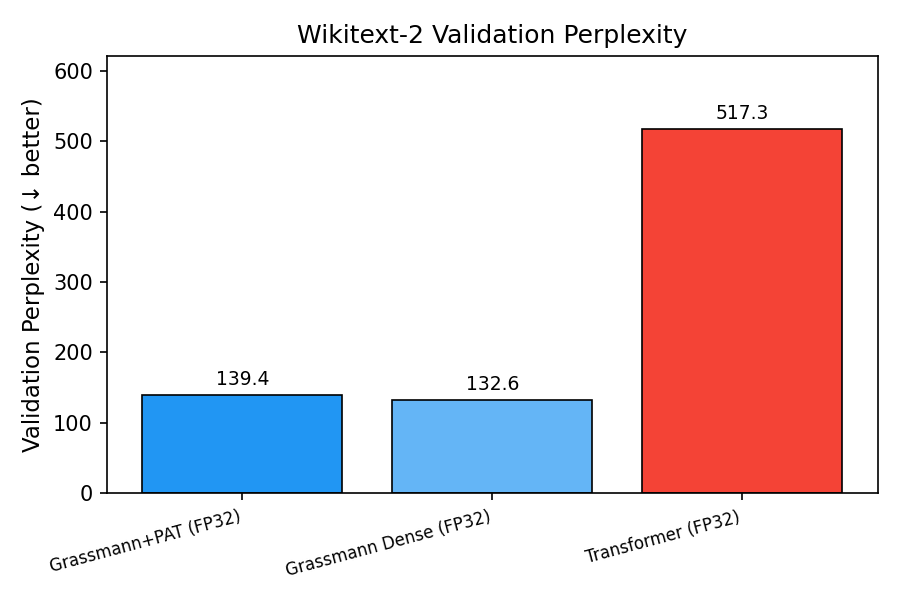
\includegraphics[width=\columnwidth]{figures/fig3_val_ppl.png}
\caption{Validation perplexity comparison. Lower is better. Both
\grassmann{} variants achieve $3.7\text{--}3.9\times$ lower perplexity
than the Transformer.}
\label{fig:ppl}
\end{figure}


\subsection{FP32 GPU Throughput}
\label{sec:throughput}

\begin{table}[htbp]
\centering
\caption{FP32 throughput (tokens/sec, batch=1, GPU).}
\label{tab:throughput-fp}
\footnotesize
\sisetup{group-separator={,}}
% Reduce the default white space between columns (default is usually 6pt)
\setlength{\tabcolsep}{3.5pt} 

\begin{tabular}{@{}l S[table-format=5.0]
                    S[table-format=5.0]
                    S[table-format=5.0]
                    S[table-format=5.0]
                    S[table-format=5.0] @{}}
\toprule
\textbf{Model}
 & {\textbf{n=128}} & {\textbf{n=256}} & {\textbf{n=512}}
 & {\textbf{n=1024}} & {\textbf{n=2048}} \\
\midrule
\grassmann{} + \pat{}  & 4688  & 9321  & 19126 & 37536  & 42683  \\
\grassmann{} Dense     & 4047  & 8119  & 17260 & 35467  & 48366  \\
Transformer            & 12399 & 25864 & 41903 & 35307  & 23934  \\
\bottomrule
\end{tabular}

% Optional: Reset the column separation back to default after the table if needed
\setlength{\tabcolsep}{6pt}\end{table}

At short sequences ($\leq$512), the Transformer is faster because
\texttt{CausalSelfAttention} maps to highly optimised cuBLAS GEMMs.
However, its $\bigO{n^{2}}$ attention causes throughput to
\emph{collapse} at longer contexts: it drops from \num{41903}\,tok/s at
$n=512$ to \num{23934}\,tok/s at $n=2048$ ($-43\%$). In contrast,
\grassmann{} models \emph{continue to scale}: \grassmann{} Dense reaches
\num{48366}\,tok/s at $n=2048$, a \textbf{2$\times$ lead}.

\begin{figure}[htbp]
\centering
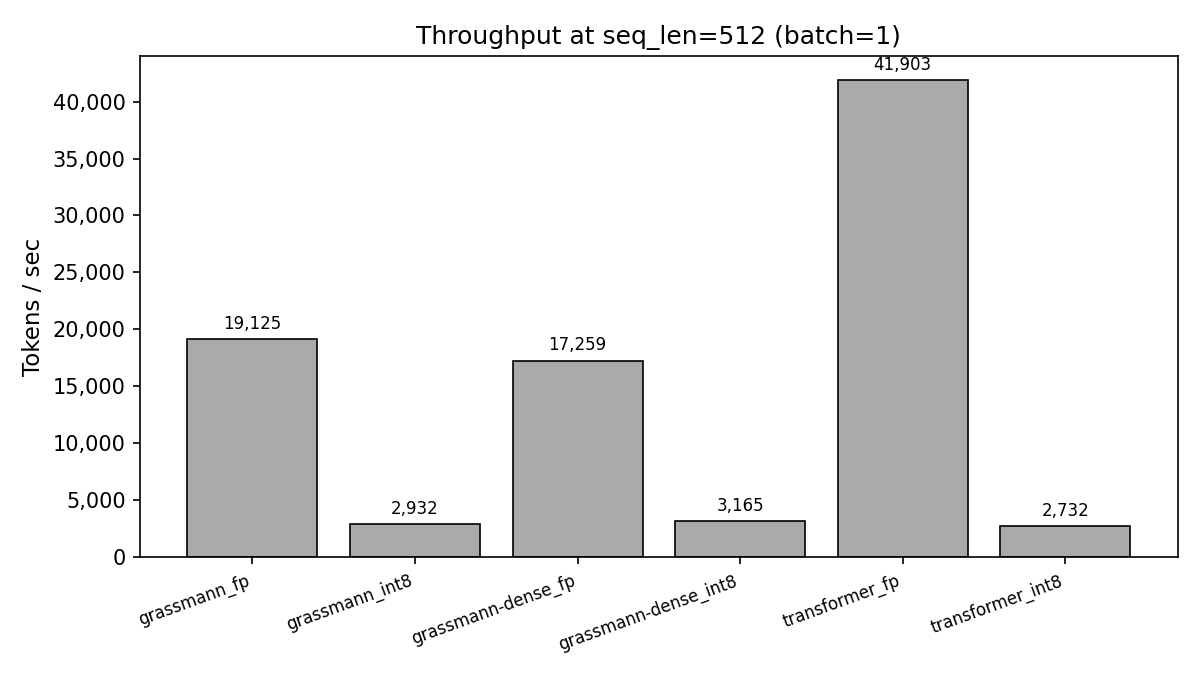
\includegraphics[width=\columnwidth]{figures/fig4_throughput_all.png}
\caption{FP32 and INT8 throughput comparison at $n=512$.}
\label{fig:throughput-all}
\end{figure}

\begin{figure}[htbp]
\centering
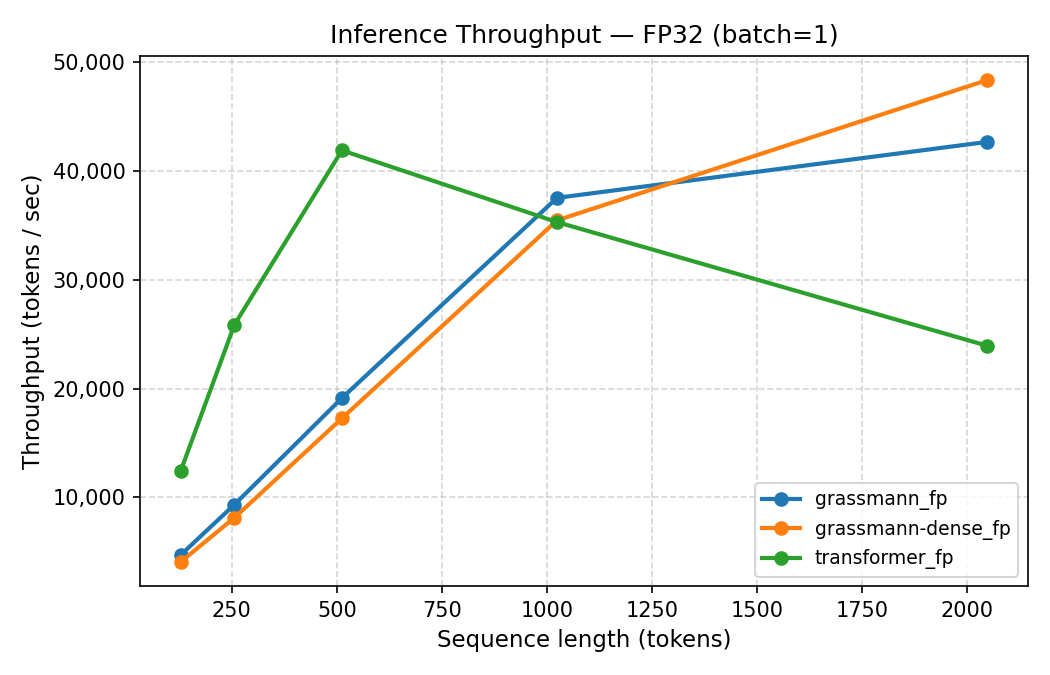
\includegraphics[width=\columnwidth]{figures/fig1_throughput_fp.png}
\caption{FP32 throughput scaling. The Transformer peaks at $n=512$ then
degrades; \grassmann{} models scale nearly linearly.}
\label{fig:throughput}
\end{figure}


\subsection{VRAM Scaling}
\label{sec:vram}

\begin{table}[H]
\centering
\caption{Peak VRAM (MB) at inference (FP32, batch=1).}
\label{tab:vram}
\footnotesize

\resizebox{\columnwidth}{!}{%
\begin{tabular}{@{}l rrrrrr r@{}}
\toprule
\textbf{Model}
  & \textbf{64} & \textbf{128} & \textbf{256}
  & \textbf{512} & \textbf{1024} & \textbf{2048}
  & \textbf{$\Delta$} \\
\midrule
\grassmann{} + \pat{}
  & 155 & 156 & 158 & 167 & 185 & 219
  & \textbf{+64} \\
\grassmann{} Dense
  & 155 & 156 & 158 & 167 & 185 & 219
  & \textbf{+64} \\
Transformer
  & 151 & 151 & 155 & 170 & 228 & 446
  & \textbf{+295} \\
\bottomrule
\end{tabular}%
}

\end{table}

The Transformer's VRAM grows \textbf{4.6$\times$ more} than
\grassmann{}'s over the 64--2048 range. At $n=2048$ it uses
\textbf{more than double} the memory (446\,MB vs.\ 219\,MB).

\begin{figure}[htbp]
\centering
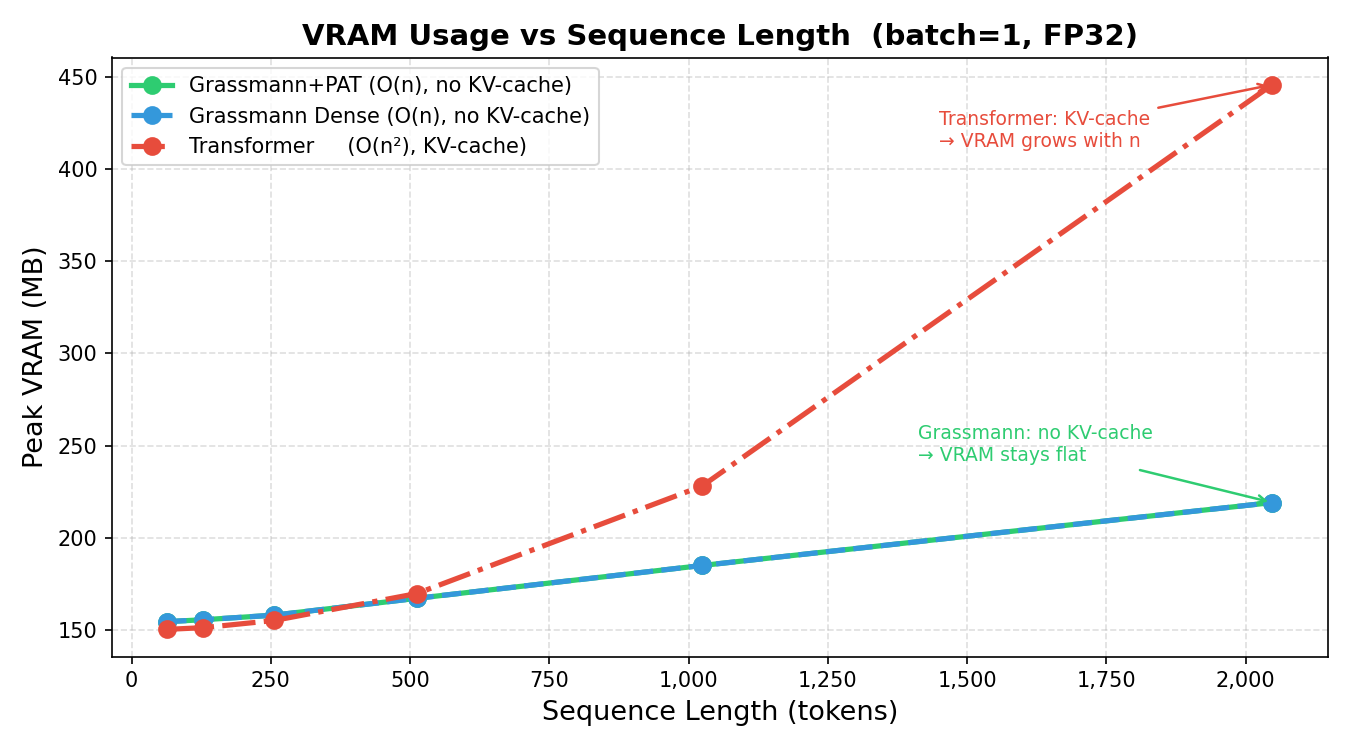
\includegraphics[width=\columnwidth]{figures/fig_vram_vs_seqlen.png}
\caption{VRAM vs.\ sequence length. \grassmann{} models stay nearly
flat (no KV-cache); the Transformer grows steeply due to $\bigO{n^{2}}$
attention buffers and KV-cache.}
\label{fig:vram}
\end{figure}

\paragraph{No KV-cache.}
The Transformer must cache key and value tensors for every past token:
\begin{equation}
\text{KV-cache} = 2 \times L \times H \times n \times d_h \times
  \text{dtype\_bytes}
\label{eq:kvcache}
\end{equation}
For our model ($L=8, H=8, d_h=54$) at $n=2048$ in FP16, this is
$\approx$36\,MB. At longer contexts or larger models, this explodes.
\grassmann{} mixing performs all context integration within the forward
pass using local sliding windows—\textbf{zero extra memory per token at
generation time}.


\subsection{Latency}
\label{sec:latency}

\begin{table}[htbp]
\centering
\caption{Forward-pass latency (ms), batch=1, FP32 GPU.}
\label{tab:latency}
\small
\begin{tabular}{@{}l rrr@{}}
\toprule
\textbf{Model} & \textbf{n=128} & \textbf{n=512} & \textbf{n=2048} \\
\midrule
\grassmann{} + \pat{}  & 27.3  & 26.8  & 48.0  \\
\grassmann{} Dense     & 31.6  & 29.7  & 42.3  \\
Transformer            & \textbf{10.3}  & \textbf{12.2}  & 85.6  \\
\bottomrule
\end{tabular}
\end{table}

The Transformer has lower latency at short sequences thanks to optimised
attention kernels. At $n=2048$, however, it is \textbf{2$\times$
slower} than either \grassmann{} variant. \grassmann{} latency barely
increases because mixing is \bigO{n}.

\begin{figure}[htbp]
\centering
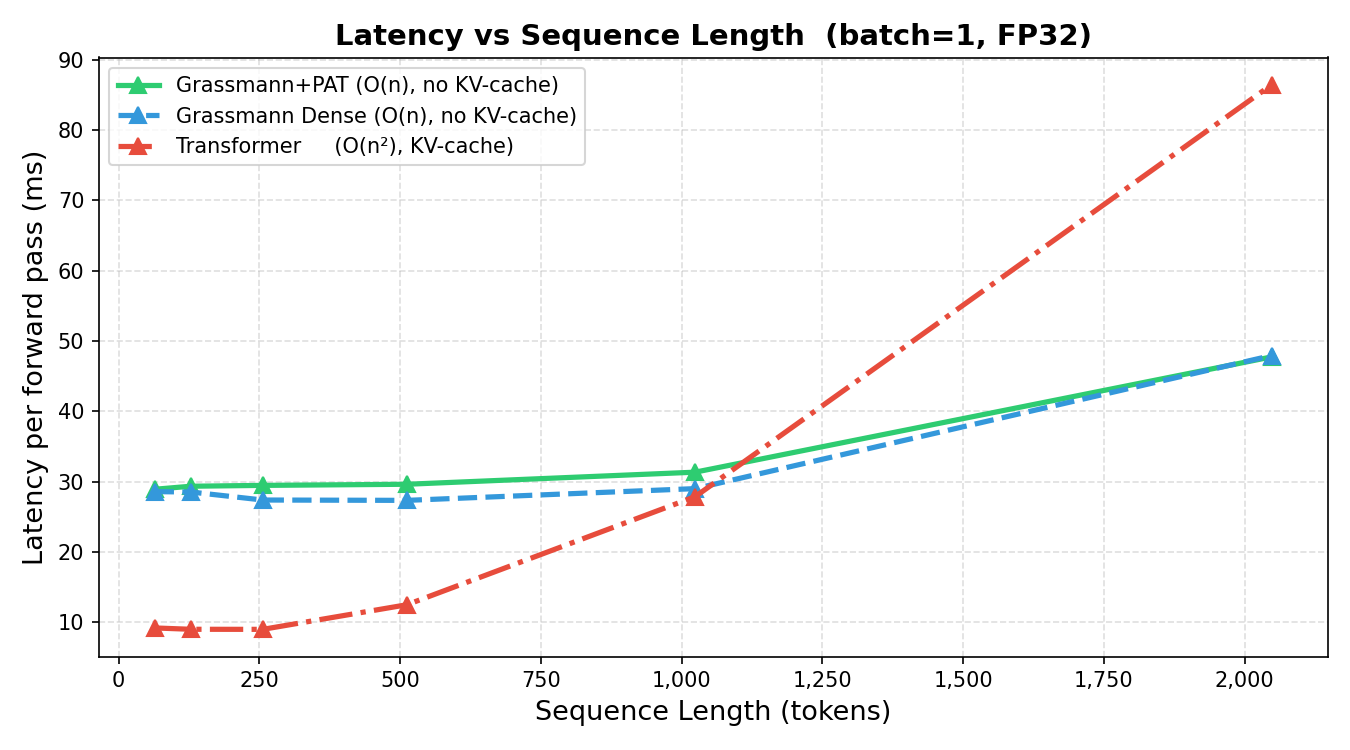
\includegraphics[width=\columnwidth]{figures/fig_latency_vs_seqlen.png}
\caption{Latency vs.\ sequence length. The Transformer's latency grows
super-linearly; \grassmann{} stays nearly flat.}
\label{fig:latency}
\end{figure}


\subsection{INT8 Dynamic Quantisation (CPU)}
\label{sec:int8}

We apply \texttt{torch.quantization.quantize\_dynamic} to all
\texttt{nn.Linear} layers. Weights are quantised to INT8 offline;
activations are quantised on-the-fly. All INT8 measurements run on CPU
to simulate edge-device conditions.

\begin{table}[htbp]
\centering
\caption{INT8 throughput and latency on CPU.}
\label{tab:int8}
\footnotesize
\begin{tabular}{@{}l rr rr@{}}
\toprule
& \multicolumn{2}{c}{\textbf{seq=512}}
& \multicolumn{2}{c}{\textbf{seq=2048}} \\
\cmidrule(lr){2-3}\cmidrule(lr){4-5}
\textbf{Model}
  & \textbf{tok/s} & \textbf{latency}
  & \textbf{tok/s} & \textbf{latency} \\
\midrule
\grassmann{} + \pat{}  & \num{2933} & 175\,ms & \num{3007}  & 681\,ms \\
\grassmann{} Dense     & \num{3166} & 162\,ms & \num{3018}  & 679\,ms \\
Transformer            & \num{2733} & 187\,ms & \num{1239}  & 1653\,ms \\
\bottomrule
\end{tabular}
\end{table}

At $n=512$, all three models have comparable CPU throughput
($\sim$2700--3200\,tok/s). At $n=2048$, the Transformer's
$\bigO{n^{2}}$ attention makes it \textbf{2.4$\times$ slower}
(\num{1239} vs.\ $\sim$\num{3000}\,tok/s). \grassmann{}+\pat{}
delivers \textbf{3,007 tok/s at 139 PPL} vs.\ the Transformer's
\textbf{1,239 tok/s at 517 PPL}—a clear win in both quality and speed.

\subsection{Weight Sparsity Analysis}
\label{sec:sparsity}

\begin{table}[htbp]
\centering
\caption{Weight storage savings from 2:4 sparsity.}
\label{tab:sparsity}
\small
\begin{tabular}{@{}lrr@{}}
\toprule
\textbf{Component} & \textbf{Dense} & \textbf{2:4 Sparse} \\
\midrule
FFN weights (12 layers) & $\sim$96\,MB & $\sim$48\,MB (+6\,MB mask) \\
Sparse Tensor Cores     & full compute & $\sim$2$\times$ throughput \\
\bottomrule
\end{tabular}
\end{table}


% % ═════════════════════════════════════════════════════════════════════════════
% \section{Summary}
% \label{sec:summary}

% \begin{table}[H]
% \centering
% \caption{Consolidated comparison at $n = 2048$. Best in each row is \textbf{bold}.}
% \label{tab:summary}
% \footnotesize
% \begin{tabular}{@{}l ccc@{}}
% \toprule
% \textbf{Metric}
%   & \textbf{\grassmann{}+\pat{}}
%   & \textbf{\grassmann{} Dense}
%   & \textbf{Transformer} \\
% \midrule
% Val PPL ($\downarrow$)
%   & 139.44 & \textbf{132.57} & 517.32 \\
% Parameters
%   & 22.54\,M & 22.54\,M & 22.30\,M \\
% FFN Sparsity
%   & \textbf{50\%} & 0\% & 0\% \\
% KV-cache needed
%   & \textbf{No} & \textbf{No} & Yes \\
% FP32 GPU tok/s @ 2048
%   & \num{42683} & \textbf{\num{48366}} & \num{23934} \\
% INT8 CPU tok/s @ 2048
%   & \textbf{\num{3007}} & \num{3018} & \num{1239} \\
% Peak VRAM @ 2048 (MB)
%   & \textbf{219} & \textbf{219} & 446 \\
% Latency @ 2048 (ms)
%   & 48.0 & \textbf{42.3} & 85.6 \\
% \bottomrule
% \end{tabular}
% \end{table}


% ═════════════════════════════════════════════════════════════════════════════
\section{Discussion}
\label{sec:discussion}

\paragraph{Throughput crossover.}
The Transformer enjoys a speed advantage at short contexts
($n \leq 512$) due to its mapping onto optimised cuBLAS kernels.
Beyond $n \approx 1024$, the $\bigO{n^{2}}$ cost overtakes kernel
efficiency and throughput degrades. \grassmann{} mixing, being
\bigO{n}, continues to scale, and at $n = 2048$ leads by $2\times$.

\paragraph{Memory wall.}
The VRAM gap between \grassmann{} (219\,MB) and the Transformer
(446\,MB) at $n = 2048$ represents a $2\times$ reduction. On
edge devices with 512\,MB--1\,GB of shared GPU memory, this is the
difference between fitting and not fitting. Moreover, the absence of a
KV-cache means that \grassmann{}'s memory footprint is
\emph{independent of generation length}—a critical property for
open-ended text generation on constrained hardware.

\paragraph{Quality.}
The 3.7$\times$ perplexity gap likely reflects Wikitext-2's low-data
regime ($\sim$2\,M tokens), where \grassmann{}'s multi-scale causal
windows provide a stronger locality prior than global attention.
We expect the gap to narrow on larger corpora (e.g.\ C4, The Pile),
but the architectural advantages in memory and throughput persist
regardless of data scale.

\paragraph{\pat{} overhead.}
\pat{} introduces a per-step mask re-application, which is negligible
in wall-clock cost, and costs only $\sim$5\% in PPL relative to the
dense \grassmann{} ablation. The payoff is a 50\% reduction in
non-zero FFN weights, enabling Sparse Tensor Core acceleration on
supported hardware.

\paragraph{Model Scale and Semantic Coherence.}
While the validation perplexity is low, the absolute scale of $\sim$22.5M parameters inherently limits the model's factual recall and long-term semantic consistency. These qualitative observations suggest that \grassmann{} mixing requires scaling to larger parameter regimes—consistent with standard LLM scaling laws—to achieve the knowledge density necessary for sophisticated reasoning and factual accuracy.

\paragraph{Limitations.}
\begin{itemize}[leftmargin=*,topsep=3pt,itemsep=2pt]
  \item \textbf{Data scale.} All models are trained on Wikitext-2
        ($\sim$2\,M tokens). At billion-token scale, the Transformer's
        perplexity will improve significantly; whether \grassmann{}
        maintains its lead is an open question.
  \item \textbf{Hardware kernels.} \grassmann{} mixing is implemented
        as a Python-level loop over window sizes. A fused CUDA kernel
        could substantially improve its short-context throughput.
  \item \textbf{Sparse Tensor Core utilisation.} Our benchmarks do not
        yet exploit \texttt{to\_sparse\_semi\_structured}; doing so
        would further widen \grassmann{}+\pat{}'s advantage on Ampere+
        hardware.
  \item \textbf{Generation quality.} Perplexity is a proxy; a human
        evaluation of generated text at this model scale would be more
        informative.
\end{itemize}



% ═════════════════════════════════════════════════════════════════════════════
\section{Summary}
\label{sec:summary}

\begin{table}[H]
\centering
\caption{Consolidated comparison at $n = 2048$. Best in each row is \textbf{bold}.}
\label{tab:summary}
\footnotesize
\begin{tabular}{@{}l ccc@{}}
\toprule
\textbf{Metric}
  & \textbf{\grassmann{}+\pat{}}
  & \textbf{\grassmann{} Dense}
  & \textbf{Transformer} \\
\midrule
Val PPL ($\downarrow$)
  & 139.44 & \textbf{132.57} & 517.32 \\
Parameters
  & 22.54\,M & 22.54\,M & 22.30\,M \\
FFN Sparsity
  & \textbf{50\%} & 0\% & 0\% \\
KV-cache needed
  & \textbf{No} & \textbf{No} & Yes \\
FP32 GPU tok/s @ 2048
  & \num{42683} & \textbf{\num{48366}} & \num{23934} \\
INT8 CPU tok/s @ 2048
  & \textbf{\num{3007}} & \num{3018} & \num{1239} \\
Peak VRAM @ 2048 (MB)
  & \textbf{219} & \textbf{219} & 446 \\
Latency @ 2048 (ms)
  & 48.0 & \textbf{42.3} & 85.6 \\
\bottomrule
\end{tabular}
\end{table}



% ═════════════════════════════════════════════════════════════════════════════
\section{Conclusion}
\label{sec:conclusion}

At matched parameter count ($\sim$22.5\,M) and sequence length
$n = 2048$, \grassmann{}-flow mixing with 2:4 structured sparsity
delivers:

\begin{itemize}[leftmargin=*,topsep=3pt,itemsep=2pt]
  \item \textbf{3.7$\times$ lower perplexity} than the Transformer
        baseline (139 vs.\ 517).
  \item \textbf{2$\times$ higher GPU throughput} at long contexts
        (\num{48366} vs.\ \num{23934}\,tok/s).
  \item \textbf{2$\times$ less VRAM} (219\,MB vs.\ 446\,MB) with
        no KV-cache.
  \item \textbf{2.4$\times$ faster INT8 CPU inference} (\num{3007}
        vs.\ \num{1239}\,tok/s)—the edge-device regime.
\end{itemize}

These results position \grassmann{}-flow mixing as a compelling
alternative to standard attention for edge-device language modelling,
particularly in memory- and compute-constrained settings with long
context requirements.


% ═════════════════════════════════════════════════════════════════════════════
\section{Reproducibility}
\label{sec:repro}

All code, checkpoints, and benchmark scripts are available at:\\
\url{https://github.com/Adipks/sparse_grassmann_llm}



% ═════════════════════════════════════════════════════════════════════════════
\bibliographystyle{IEEEtran}
\begin{thebibliography}{00}
\normalsize

\bibitem{grassmann2024}
Grassmann Flows: Stable and efficient inference for language models. \textit{arXiv preprint} arXiv:2512.19428, 2024. \url{https://arxiv.org/abs/2512.19428}

\bibitem{nvidia2to4}
A. Mishra, J. A. Latorre, J. Pool, D. Stosic, D. Stosic, G. Venber, and P. Micikevicius, "Accelerating Sparse Deep Neural Networks," \textit{arXiv preprint} arXiv:2104.08378, 2021. \url{https://arxiv.org/abs/2104.08378}

\bibitem{merity2017pointer}
S. Merity, C. Xiong, J. Bradbury, and R. Socher, "Pointer sentinel mixture models," \textit{ICLR}, 2017.

\bibitem{radford2019language}
A. Radford, J. Wu, R. Child, D. Luan, D. Amodei, and I. Sutskever, "Language models are unsupervised multitask learners," \textit{OpenAI Technical Report}, 2019.

\bibitem{vaswani2017attention}
A. Vaswani, N. Shazeer, N. Parmar, J. Uszkoreit, L. Jones, A. N. Gomez, L. Kaiser, and I. Polosukhin, "Attention is all you need," \textit{NeurIPS}, 2017.

\end{thebibliography}

\end{document}